\documentclass{article}
\usepackage[utf8]{inputenc}
\usepackage{booktabs,caption}
\usepackage[flushleft]{threeparttable}
\usepackage{natbib}
\usepackage{url}
\usepackage{graphicx}

\title{FAIR from metadata to the Semantic Web: open source services for data annotation and findable data}
\author{TBD}
\date{November 2019}

\begin{document}

\maketitle

\begin{abstract}
Annotation of research data with metadata is crucial to provide context for analysis and  re-use. The odML format offers a flexible and comprehensive solution for the scientist to collect and organize metadata in a structured form that is both human readable and machine actionable for documentation and automated analysis. To further support the FAIR principles, we present tools to export metadata from odML to \textit{RDF}\footnote{\url{https://www.w3.org/TR/2014/REC-rdf11-concepts-20140225}}, which opens any metadata to \textit{Semantic Web}\footnote{\url{https://www.w3.org/standards/semanticweb}} services. The open source G-Node SPARQL server is aimed at providing searchable whole metadata sets for meta analyses and also providing links to the actual published scientific data set. Scientists can upload their metadata to make their data findable and accessible even if it was a data publication or if it is an unpublished data set.
\end{abstract}

\section{Introduction}
According to the FAIR principles \cite{Wilkinson_2016}, (meta)data is supposed to be Findable, Accessible, Interoperable, Reusable. Metadata, data about experimental data, play a special role in this context. Not only do they accurately describe the experimental setup but ideally also the dataset involved. If handled properly, a collection of metadata is the first step to solving the FAIR principles for a dataset. As previously shown \cite{Teeters_2017} Interoperability  between even diverse metadata can be achieved by using the common and flexible Semantic Web RDF technology.
Expanding on this idea, we show how Findability and Accessibility of large collections of metadata can be achieved by the use of open source software. Interoperability between different types of metadata is achieved by a minimal set of common RDF terms. This way diverse sets of metadata can be easily converted and imported into a common searchable data graph. Taking advantage of the powerful OWL feature of RDF, each distinct set of metadata can be subclassed to the benefit of maintaining the original structure without losing the common generic structure keeping Interoperability without sacrificing Findability.
To make large collections of merged metadata in RDF format easily Accessible, we introduce an augmented version of the open source SPARQL server \textit{Apache Fuseki}\footnote{Jena 2006, A semantic web framework for Java, \url{http://jena.apache.org}}. This software provides access to the metadata by both custom, easy to use search terms as well as the powerful \textit{SPARQL}\footnote{\url{https://www.w3.org/TR/sparql11-query}} query language.

\subsection{The odML data format}
As previously reported \cite{Grewe_2011}, \textit{odML}\footnote{\url{https://github.com/G-Node/python-odml}, RRID:SCR\_001376} is a data format designed to thoroughly document diverse metadata that comes with a freely available reference implementation in Python. Developed by the German Neuroinformatics Node, its design was oriented along the needs of Neuroscientific metadata, but its generic approach makes it applicable to any scientific field and is able to store heterogenic metadata to fully document even complex experimental setups and conditions \cite{Zehl_2016}.
As a brief introduction to the odML concept is to store metadata in a generic but hierarchical structure. Figure ~\ref{fig:odmlModel}A provides an overview of the general odml data model with all its available attributes while Fig[odmlModelB] shows an abstraction of how the model can be used to store metadata.

\begin{figure}
\begin{center}
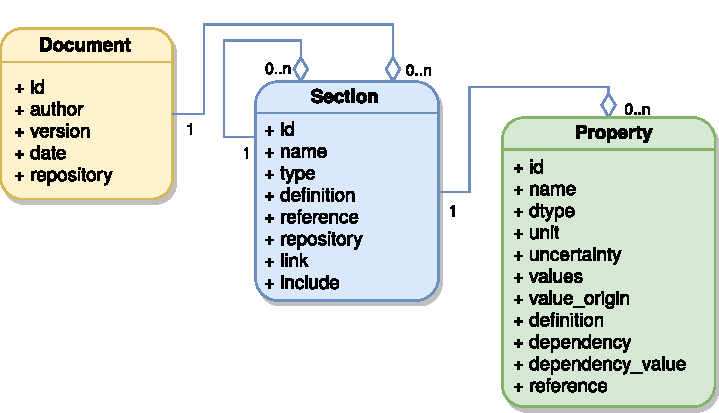
\includegraphics[width=0.70\columnwidth]{figures/figOdmlModelA.pdf}
\caption{
A) The odML data model. B) [xxx todo] The two main concept entities are nested *Sections* that provide a single *Document* with its general structure an make such a document navigate- and searchable. *Sections* can contain *Properties* that in turn contain metadata values.
}
\label{fig:odmlModel}
\end{center}
\end{figure}

Metadata organized using the odML data model can be stored in multiple different file formats: XML, JSON and YAML. See Fig[formatExamples] for examples. While both XML and JSON are well used in data processing and automation, YAML provides an option for both human readability and machine consumption.
Fig[formatExamples]. Metadata organized in odML and stored using the XML[formatExamplesA], JSON[formatExamplesB] and YAML[formatExamplesC] storage formats.
We used parts of the datacite schema as an example since it will serve later on as one of the main search criteria to find and link back to published or otherwise available datasets. We provide a full DataCite odML terminology \footnote{\url{https://terminologies.g-node.org/v1.1/datareference/datacite.xml}}, two specific odML templates \footnote{\url{https://templates.g-node.org/datacite/datacite.crcns.xml}, \url{https://templates.g-node.org/datacite/datacite.gnode.xml}} as reference usage implementation and a Python conversion script from XML Datacite files to odML \footnote{[xxx] TBD}.

\subsection{Further development to open odML to graph database searches}

While odML has shown to document experiments even through diverse fields due to its flexibility, there is a growing need to search metadata across multiple experiments and even across multiple fields. As recently published \cite{Sprenger_2019}, the odML data format has been developed further to also address this growing demand.

Even though searches within even extensive odML documents were always part of the implementation and even imports from linked, external sources into individual documents are possible, the option to easily search across multiple documents was still lacking. To this end we chose to open the odML data format to the \textit{Semantic Web}\footnote{\url{https://www.w3.org/standards/semanticweb}} via conversion to the \textit{RDF (Resource Description Framework)}\footnote{\url{https://www.w3.org/TR/2014/REC-rdf11-concepts-20140225}} format.

The Semantic Web offers a large technology stack fit to meet the requirements: A suite of various graph database tools to merge individual documents in the RDF format into a single graph even if the content of the documents are not uniform. SPARQL (SPARQL Protocol and RDF Query Language), a full fledged query language that can be used to extract information from such a graph. Another feature is \textit{OWL (Web Ontology Language)}\footnote{\url{https://www.w3.org/TR/owl-ref}} which enables the definition of a vocabulary extension of the basic RDF terminology to enable more elaborate and domain specific SPARQL searches. The broad range of freely available open source tools can be adapted to fit more specific use cases.

\section{Implementation}

In the following we will describe how we mapped the versatile odML data format to its RDF equivalent and document the specific OWL ontology we devised. We will also show how metadata can be exported from odml to its rdf equivalent, how different documents can be loaded into a single graph and how it can be searched via SPARQL.
We will show how the basic structure can be furthered with indidual subclasses to make searches more specific.
Finally we will present an open web service that enables metadata searches across multiple documents and present a suggestion based on the widely accepted \textit{DataCite}\footnote{\url{https://datacite.org}} publication standard to enable backlinks from metadata sets to the original, published data.

\subsection{Implementation of odML to RDF mapping}

First step was mapping the odML entities `Document`, `Section` and `Property` to RDF classes and provide the respective RDF predicates and xsd types.

\subsubsection{Namespace}

We chose the RDF namespace `https://g-node.org/projects/odml-rdf` to identify all RDF odML entities. [xxx should we change this namespace? if yes to what should we change it and we need to provide the odML OWL ontology at this namespace in any case, cf. related section below]

\subsubsection{Mapping of odML entities to RDF classes}

In the following we descript how odML entities were mapped to RDF.

\begin{table}
\begin{threeparttable}
\caption{odML Document}
\begin{tabular}{l|l|l}
    odml                    & RDF                                 & xsd type \\
\hline
    odml (a)                & odml:Document                       & - \\
                            & & \\
    id (b)                  & RDF node instance name              & - \\
    author                  & odml:hasAuthor                      & xsd:string \\
    date                    & odml:hasDate                        & xsd:date \\
    version (odml)          & odml:hasVersion                     & xsd:float \\
    version (document)      & odml:hasDocVersion                  & xsd:string \\
    repository (c)          & odml:hasTerminology                 & - \\
                            & odml:hasExternalTerminology         & xsd:string \\
    Sections                & odml:hasSection                     & - \\
    - (d)                   & odml:hasFilename                    & xsd:string \\
\end{tabular}
\begin{tablenotes}
\small
\item Mapping of odML `Document` to RDF. (a) The document root is mapped to an RDFS class of type `odml:Document`. (b) The uuid of the odML `Document` is used as Name of the created `odml:Document` RDF node to uniquely identify the document if it is merged with a graph database. (c) RDF export of repositories: linked terminologies are downloaded on conversion and exported additional RDF document connected via the `odml:Hub` RDF node. This additional document is linked via `odml:hasTerminology` to the original document. If the terminology cannot be imported, its URL will be kept as is and its value is provided as an RDF leaf via the predicate `odml:hasExternalTerminology` in the original document. See [TableHub] and [TableTerminology] for more detailed descriptions [xxx check if this actually works as described] (d) As provenance from where the RDF odml:Document was created from, the filename of the original odML file is documented via the non-odML predicate `odml:hasFilename`.
\end{tablenotes}
\end{threeparttable}
\end{table}

\begin{table}
\begin{threeparttable}
\caption{odML Section}
\begin{tabular}{l|l|l}
    odml            & RDF                             & xsd type \\
\hline
    Section (a)     & odml:Section                    & - \\
                    & & \\
    id (b)          & RDF node instance name          & - \\
    name            & odml:hasName                    & xsd:string \\
    type            & odml:hasType                    & xsd:string \\
    definition      & odml:hasDescription             & xsd:string \\
    repository (c)  & odml:hasTerminology             & - \\
                    & odml:hasExternalTerminology     & xsd:string \\
    reference (d)   & odml:hasReference               & xsd:string \\
    Sections (e)    & odml:hasSection                 & - \\
    Properties      & odml:hasProperty                & - \\

\end{tabular}
\begin{tablenotes}
\item Mapping of odML `Section` to RDF. (a) Any odML `Section` entity is mapped to an RDFS class of type `odml:Section`. (b) The uuid of an odML `Section` entity is used as Name of the created `odml:Section` RDF node to uniquely identify the section if it is merged with a graph database. If this node already exists in the graph, it will not add a duplicate entry, but will add only any predicates that the graph with respect to this Section node does not already contain. [xxx Move to another part or remove?] (c) cf. `repository` description in [TableDocument]. (d) A `reference` can either be be a URL to an external reference or a string pointing to an id in a Database. (e) Unspecific Sections are exported using the `odml:Section` class and the `odml:hasSection` predicate. We also provide a set of 'specialized' RDF classes that are subclasses of Section. cf. [subclassing] for details.
\end{tablenotes}
\end{threeparttable}
\end{table}

\begin{table}
\begin{threeparttable}
\caption{odML Property}
\begin{tabular}{l|l|l}
    odml            & RDF                             & xsd type \\
\hline
    Property (a)    & odml:Property                   & - \\
                    & & \\
    id (b)          & RDF node instance name          & - \\
    name            & odml:hasName                    & xsd:string \\
    definition      & odml:hasDefinition              & xsd:string \\
    reference (c)   & odml:hasReference               & xsd:string \\
    unit            & odml:hasUnit                    & xsd:string \\
    dtype           & odml:hasDtype                   & xsd:string \\
    uncertainty     & odml:hasUncertainty             & xsd:float \\
    values (d)      & odml:hasValue                   & - \\
                    & rdf:Seq                         & - \\
                    & rdf:_#                          & xsd:string \\
    value_origin    & odml:hasValueOrigin             & xsd:string \\
\end{tabular}
\begin{tablenotes}
\item mapping of odML `Property` to RDF. (a) Any odML `Property` entity is mapped to an RDFS class of type `odml:Property`. (b) The uuid of an odML `Property` entity is used as Name of the created `odml:Property` RDF node to uniquely identify the section if it is
merged with a graph database. (c) cf. `reference` description in [TableSection]. (d) odML supports multiple values. On the export to RDF the order of these values need to be respected as well. Values are connected to the RDF document via the `odml:hasValue` predicate to an `rdf:Seq` node. This `rdf:Seq` node in turn contains numbered rdf:li items which in turn contain the individual odml.Value entries. This construct enables RDF searches for individual values rather then searching for lists of values.
\end{tablenotes}
\end{threeparttable}
\end{table}

\begin{table}
\begin{threeparttable}
\caption{Hub}
\begin{tabular}{l|l|l}
    odml            & RDF                           & xsd type \\
\hline
    -               & odml:Hub                      & - \\
    -               & odml:hasDocument              & - \\
    -               & odml:hasTerminology           & - \\
\end{tabular}
\begin{tablenotes}
\item The custom RDF type of class `odml:Hub` has no odML entity equivalent. It is introduced to merge Documents and Terminologies into a single RDF graph: the `Hub` is used to root a graph that might contain multiple documents to enable searches across unrelated and inhomogenious metadata content.
\end{tablenotes}
\end{threeparttable}
\end{table}

\begin{table}
\begin{threeparttable}
\caption{Terminology}
\begin{tabular}{l|l|l}
    odml            & RDF                               & xsd type \\
\hline
    -               & odml:Terminology                  & - \\
    Sections        & odml:hasSection                   & - \\

\end{tabular}
\begin{tablenotes}
\item odML documents can link to external Terminology documents. To make these available for searches within a connected RDF graph besides the odML documents they are referenced by, linked terminologies are imported and converted into RDF documents. They are connected via the `odml:hasSection` predicate to their referencing documents. Conversely the odml:Section in an odml:Document references the Terminology via the `odml:hasTerminology` predicate.
\end{tablenotes}
\end{threeparttable}
\end{table}

\begin{figure}
\begin{center}
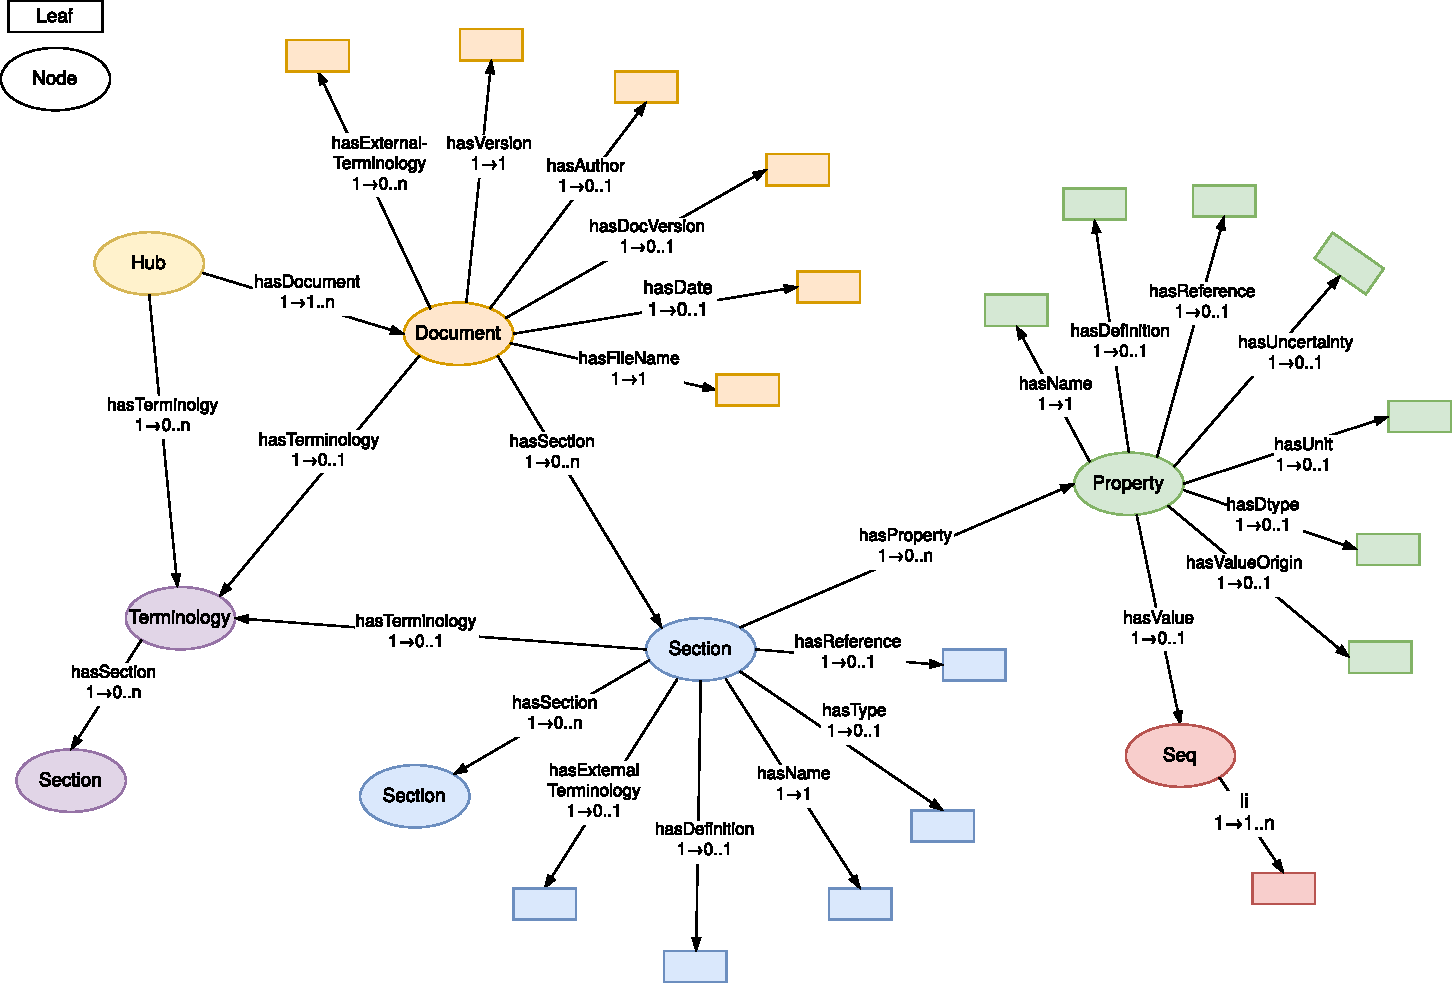
\includegraphics[width=0.90\columnwidth]{figures/odmlRDFDataModel.pdf}
\caption{The odML RDF data model.}
\label{fig:rdfModel}
\end{center}
\end{figure}

\subsubsection{Subclassing of Sections}

ALL of the properties can be fine grained into subproperties to give more semantic meaning to the connection between nodes.

e.g.
    section hasSection section
 could become
    section hasExperimenter section

Here hasExperimenter is a subclass of `hasSection` ... a search for `hasExperimenter` would return only sections connected via this specific property, a search for hasSection would return all sections connected by `hasSection` and `hasExperimenter`.

\subsubsection{odML RDF ontology}
To make use of the RDF feature of validating individual RDF files, we created an odML RDF ontology which includes the basic set of odml RDF terms and included all currently supported Section subclasses. This list of subclasses should not be seen as permanent and
will probably increase in the future.

[odmlOntology][odml-ontology.ttl] cf file. [xxx how to best include this file in the article]

\subsection{Implementation of SPARQL server: meta.g-node.org}

Fuseki is an open source SPARQL query server from the \textit{Apache Jena}\footnote{Jena 2006, A semantic web framework for Java, \url{http://jena.apache.org}} Semantic Web tools suite that was adopted to support odML specific RDF. A publicly accessible instance is available at https://meta.g-node.org. The service provides a metadata graph searchable by SPARQL containing all scientific Datasets that have been published by \textit{CRCNS (Collaborative Research in Computational
Neuroscience)}\footnote{\url{https://crcns.org}} and \textit{G-Node}\footnote{\url{https://doid.gin.g-node.org}}. The server provides example SPARQL queries how the available database can be used. The service is free to use and free to contribute, any additions to the database are welcome and encouraged.
The SPARQL server including all example queries has been Dockerized. Both source code\footnote{\url{https://github.com/G-node/odml-query}} and docker container\footnote{\url{https://hub.docker.com/r/gnode/meta}} are freely available and free to use.

\subsection{Suggested workflow}

\begin{figure}
\begin{center}
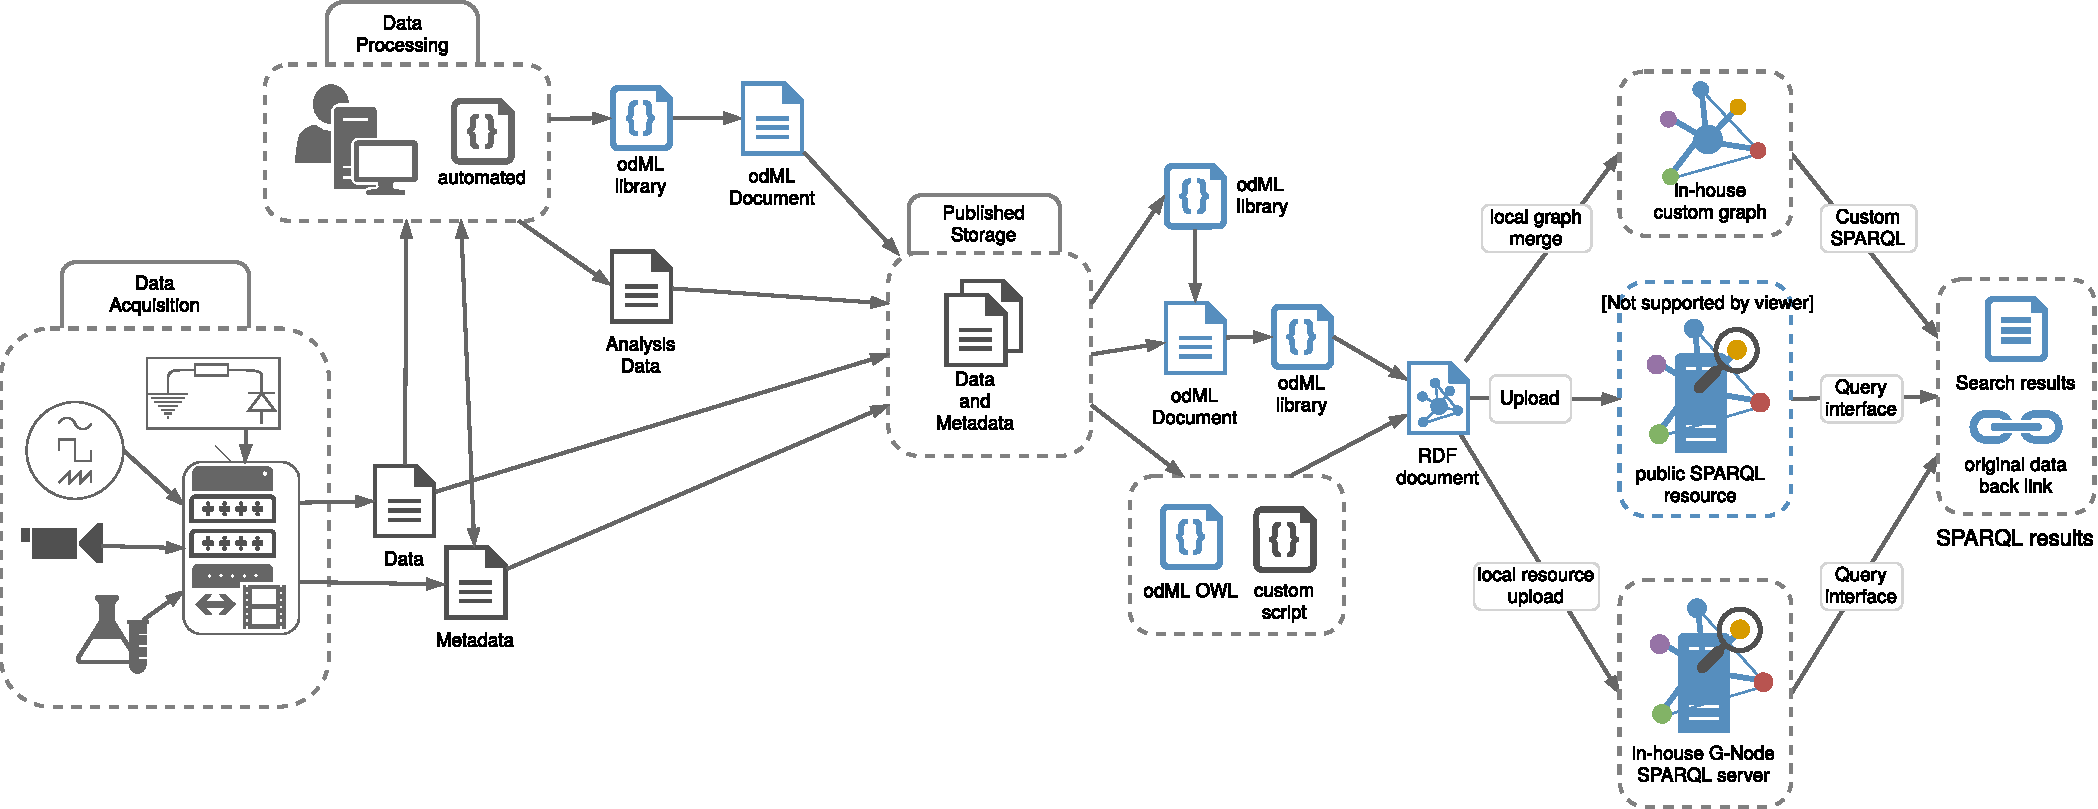
\includegraphics[width=0.90\columnwidth]{figures/workflowSchema.pdf}
\caption{Should we add a suggested workflow? Could be an adopted figure from INCF 2018/2019 from recording to graph server.}
\label{fig:workflowSchema}
\end{center}
\end{figure}

\subsection{odML for backlink}
- datacite port to odML template
- other odML templates for making datasets findable via the server

\section{Outlook}
Custom subclassing
Integration into GIN for automatic upload

\begin{thebibliography}{}
\bibitem{Grewe_2011}
Grewe J., Wachtler T., and Benda J. (2011). A bottom-up approach to data annotation in neurophysiology. Front. Neuroinform. 5:16, doi: 10.3389/fninf.2011.00016
\bibitem{Zehl_2016}
Zehl L., Jaillet F., Stoewer A., Grewe J., Sobolev A., Wachtler T., Brochier G., Riehle A., Denker M., Grün S. (2016). Handling Metadata in a Neurophysiology Laboratory. Frontiers in Neuroinformatics 10:26, doi: 10.3389/fninf.2016.00026
\bibitem{Wilkinson_2016}
Wilkinson M.D., Dumontier M., Aalbersberg I.J., Appleton G., Axton M., Baak A., Blomberg N., Boiten J., da Silva Santos L.B., Bourne P.E., Bouwman J., Brookes A.J., Clark T., Crosas M., Dillo I., Dumon O., Edmunds S., Evelo C.T., Finkers R., Gonzalez-Beltran A., Gray A.J.G., Groth P., Goble C., Grethe J.S., Heringa J., ’t Hoen P.A.C, Hooft R., Kuhn T., Kok R., Kok J., Lusher S.J., Martone M.E., Mons A., Packer A.L., Persson B., Rocca-Serra P., Roos M., van Schaik R., Sansone S., Schultes E., Sengstag T., Slater T., Strawn G., Swertz M.A., Thompson M., van der Lei J., van Mulligen E., Velterop J., Waagmeester A., Wittenburg P., Wolstencroft K., Zhao J., Mons B. (2016). The FAIR Guiding Principles for scientific data management and stewardship, Scientific Data 3:160018, doi: 10.1038/sdata.2016.18
\bibitem{Sprenger_2019}
Sprenger J, Zehl L, Pick J, Sonntag M, Grewe J, Wachtler T, Grün S and Denker M (2019). odMLtables: A User-Friendly Approach for Managing Metadata of Neurophysiological Experiments. Front. Neuroinform. 13:62, doi: 10.3389/fninf.2019.00062
\bibitem{Teeters_2017}
Teeters J.L., Ježek P., Garbers C., Kellner C.J., Sonntag M., Koutsou A., Grewe J., Sommer F.T., Wachtler T., Towards interoperability of neurophysiology data repositories, doi: 10.12751/incf.ni2017.0017
\end{thebibliography}

\end{document}
